\documentclass[8pt,pdf,hyperref={unicode}]{beamer}
\usepackage{lmodern} 
\usepackage[T2A]{fontenc}
\usepackage[utf8]{inputenc}
\setbeamertemplate{navigation symbols}{}
\usetheme{Warsaw}
\usecolortheme{seahorse}
		\title{   Практикум на ЭВМ.\\     Задание 4}
		\institute{Московский Государственный Университет М.В Ломоносова\\
					Факультет Вычислительной математики и Кибернетики\\
						Кафедра Исследования Операций\\}
		\author{Агайдарова Айганым, 311 группа}
		\date{Москва 2018}
\begin{document}
	\begin{frame}
		\titlepage
	\end{frame}
	
	\begin{frame}	
		\frametitle{Постановка задачи}
После оглушительного успеха в освобождении Астапора, Миэрина и Юнкая от власти работорговцев Дейенерис Бурерожденная открыла себе доступ к Летнему морю, а следовательно, и путь в Вестерос.
Для ведения войны с Семью Королевствами нужно оружие (т.е.нужна сталь). Безупречные кузнецы искуссны, но на поставщики стали так надеяться нельзя.
Главными поставщиками стали являются Westeros Inc. и Harpy \& Co.
Нам предоставлен CSV-файл с данными о производстве оружия и количестве сломанного оружия за каждый месяц каждым из кузнецов.
Нам необходимо исследовать, с каким же поставщиком выгодно и надежно будет заключить договор о поставках?
	\end{frame}
	
	\begin{frame}
		\frametitle{ Описание решения задачи }
		\begin{itemize}
		\item Мы использовали несколько показателей и значений для анализа данных:\\
		\begin{enumerate}
			\item Среднее число поломок мечей обеих компаний
			\item Срок службы меча. 
			\item Количество поломок изготовленных мечей в каждом месяце.
			\item Распределение мечей, в частности, на два месяца.

		\end{enumerate}
		\end{itemize}	

		Замечание: Сравнивая компании, мы выяснили, что сталь Harpy \& Co лучше, чем сталь Westeros Inc. Однако в промежутках исследования мы смогли сделать несколько выводов, позволяющих более точно выбрать поставщика стали для успешного проведения войны.		
	\end{frame}		
		
	\begin{frame}
	\frametitle{Анализ и выводы}
	\framesubtitle{Критерий №1. Среднее число поломок}
		\begin{itemize}
			\item  Мы определили, что, ориентировочно, среднее число поломок мечей, изготовленных из стали Westeros.inc, больше за все время, при одинаковом объеме производства.
			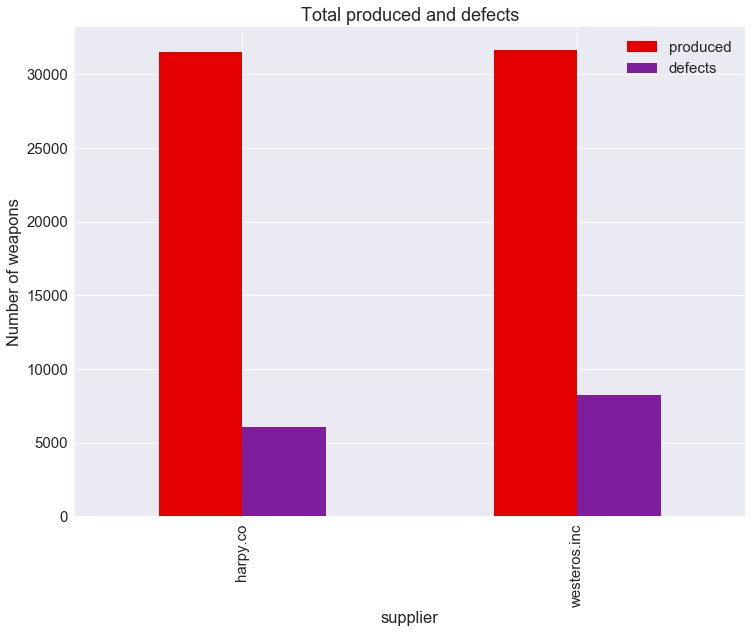
\includegraphics[scale=0.35]{1.png}
			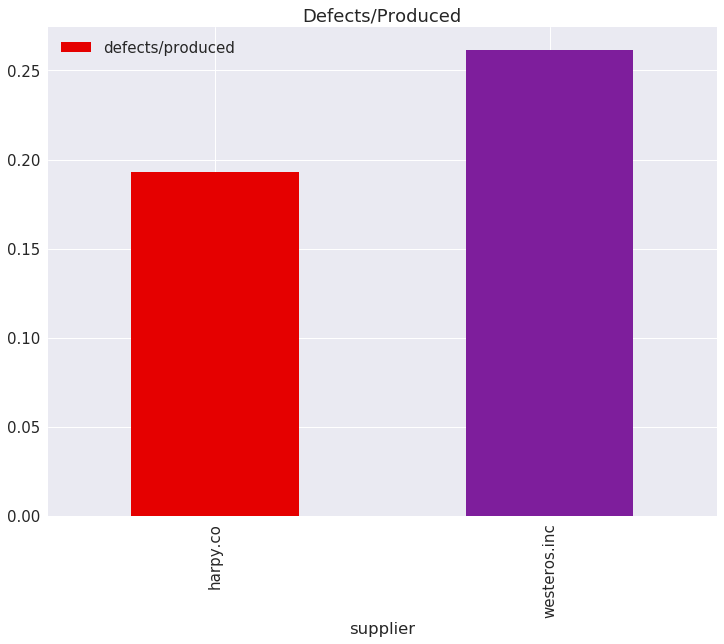
\includegraphics[scale=0.35]{2.png} 
		\end{itemize}
	\end{frame}
			
	\begin{frame}
		\frametitle{Анализ и выводы}
	\framesubtitle{Критерий №2. Срок службы меча.}
		\begin{itemize}
			\item  Число сломанных мечей из числа изначально изготовленных, в зависимости от месяца, в который они были произведены уменьшилось.
Исходя из результатов, мы можем сказать, что в период времени до 3 месяцев мечи  фирмы Harpy \& Co. стали прочнее.
Однако, на более долгий промежуток времени (более 3 месяцев), все же лучше выбрать фирму Westeros Inc., т.к. количество сломанных мечей из стали этой компании уменьшается довольно стремительно.
Но этими результатами мы можем объективно пользоваться только в случае рассмотрения определенного месяца/совокупности месяцев для закупки мечей, т.к успешность изготовления прочныз мечей в разные временные промежутки довольно резко "скачет", и этот критерий не может быть на 100\% точным. \\
			\center{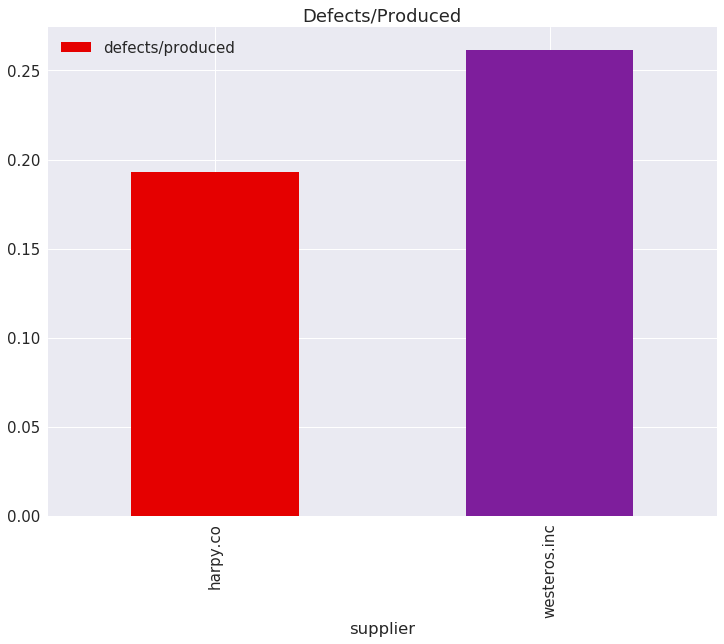
\includegraphics[scale=0.48]{2.png}}
			
		\end{itemize}
	\end{frame}
	
	\begin{frame}
	\frametitle{Анализ и выводы}
	\framesubtitle{Критерий №3. Количество поломок мечей в каждом месяце.}
	\begin{itemize}
		\item  Из графиков среднего числа сломанных мечей в каждом месяце, изображенных ниже, мы видим, что мечи из стали компании Westeros Inc. в начале ломается больше, но количество поломок уменьшается с течением времени. А мечи и стали компании Harpy \& Co. в среднем на протяжении всего рассматриваемого времени меньше, чем у первой фирмы, но, начиная с 4 месяца, количество поломок становится больше.
Это, опять же, показывает, что рассмотрение в среднем за все время и за опрделенные промежутки времени дает разные результаты\\
	
		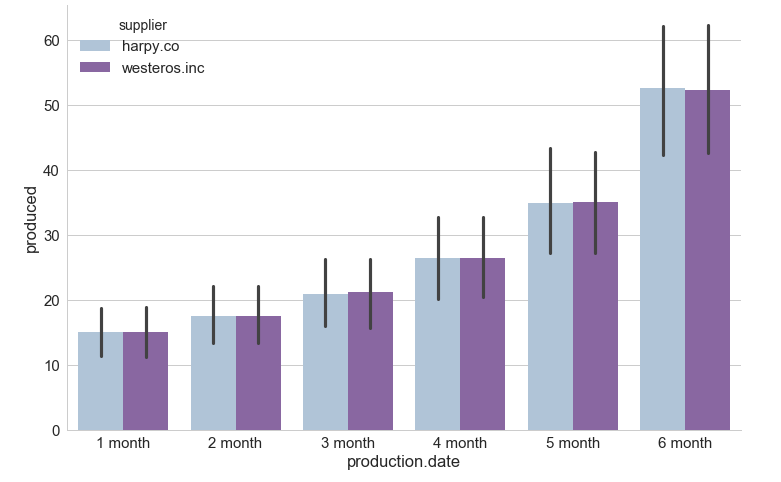
\includegraphics[scale=0.32]{3.png}		
		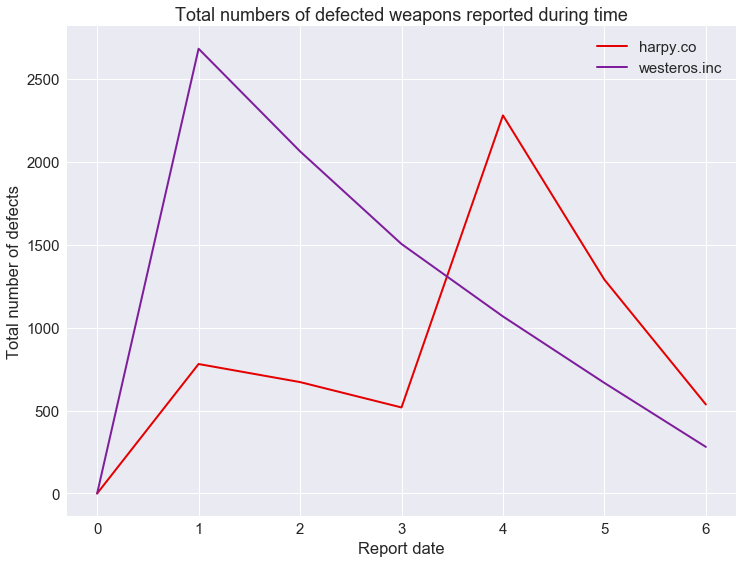
\includegraphics[scale=0.32]{4.png}	
	\end{itemize}
	\end{frame}	
	
	\begin{frame}
	\frametitle{Анализ и выводы}
	\framesubtitle{Критерий №4. Распределение мечей на два месяца}
	\begin{itemize}
		\item   Зачем нам рассматривать распределение мечей сроком на 2 месяца?
		Т.к. поставка мечей производится каждый месяц, мы можем не переживать о мечах, которые могут сломаться через продолжительное время (мы сможем их заменить вновь поставленными), а в случае, когда нам необходимо именно сейчас иметь в наличии мечи непонятно, что же делать, чтобы не уйти в минус.
Для этого мы и учитываем критерий числа поломок мечей за 2 месяца, т.е.на на каждый следующий 3-ий месяц данных у нас нет.
По графику на этом слайде можно сказать, что сталь Harpy \& Со. более надежна, а значит, что мы еще и сможем запасаться мечами на "черный день", т.к. в среднем поломок мечей из стали данной фирмы в разы меньше.  				
		\center{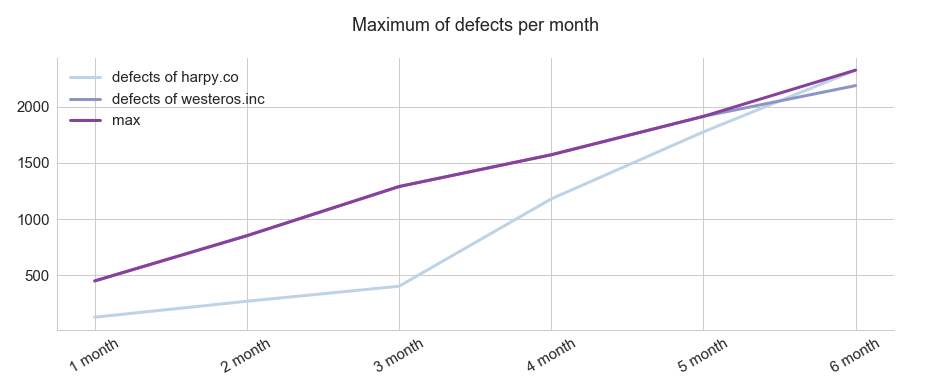
\includegraphics[scale=0.42]{5.png}}
		\end{itemize}
	\end{frame}
	\begin{frame}
	\frametitle{Вывод}
Подведем итоги:

Cталь компании Harpy\& Co. для нас надежнее, чем сталь компании

Westeros Inc. 
Однако, в отдельных случаях это может привести к провалу, т.к. сталь фирмы Harpy \& Co. имеет свойство не ломаться лишь в малые промежутки времени, поэтому это может стать проблемой для запасания мечами, а что касается минусов стали фрмы Westeros Inc., то здесь имеет место риск проигрыша войны на сегодняшний определенный день, т.к. запасы есть, но завтра они уже могут не пригодиться, т.к. война уже проиграна.
	\end{frame}
	
		\begin{frame}
		\frametitle{Работу выполняли}
		\begin{itemize}
			\item Агайдарова Айганым, 3 курс ВМК МГУ, кафедры ИО, 311 группа.\\
		\end{itemize}	
	\end{frame}
	
	
\end{document}
